\section{Problema 2: Caballos salvajes}

\subsection{Presentación del problema}
En este problema nos presentan un tablero de dimensiones conocidas pero no acotadas
del mismo tipo que el de ajedrez, es decir un tablero cuadriculado y cuadrado:\\
\begin{figure}[H]
	\begin{minipage}[t]{\linewidth}
		\centering
		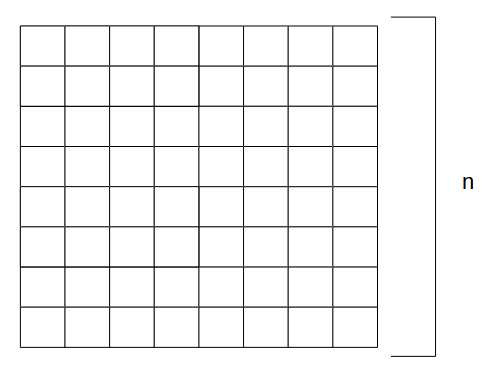
\includegraphics[scale=0.5]{show_dimension.png}
		%\caption{}
		\label{fig:p2_complejidad_varia_k}
	\end{minipage}
\end{figure}
y un conjunto de caballos, piezas de ajedrez, en casillas también conocidas, por ejemplo:\\
\begin{figure}[H]
	\begin{minipage}[t]{\linewidth}
		\centering
		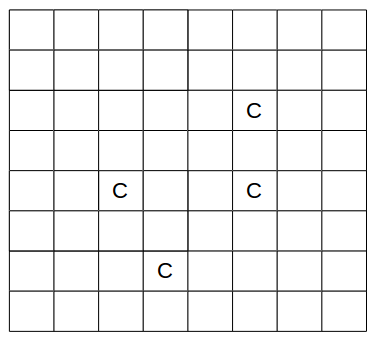
\includegraphics[scale=0.5]{show_horses.png}
		%\caption{}
		\label{fig:p2_complejidad_varia_k}
	\end{minipage}
\end{figure}
el objetivo es reunir a todos los caballos en una misma casilla del tablero con una cantidad
de movimientos total, es decir sumando los movimientos que le tomo a cada uno de los caballos, mínima.
Los movimientos permitidos a los caballos son los mismos que los impuestos por las reglas de ajedrez:\\
\begin{figure}[H]
	\begin{minipage}[t]{\linewidth}
		\centering
		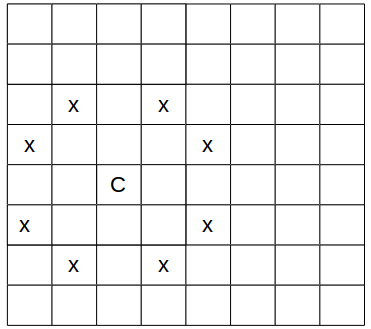
\includegraphics[scale=0.5]{show_jumps.png}
		\caption{La C representa la casilla donde está ubicado el caballo y X los lugares a los cuales podría saltar.
}
		\label{fig:p2_complejidad_varia_k}
	\end{minipage}
\end{figure}
A continuación mostramos un tablero de $4 \times 4$ en el cual los caballos comienzan en las esquinas, donde
aparecen las C pequeñas. Los números dentro de las casillas representan la suma de las distancias de los caminos
mínimos de cada uno de los caballos hasta esa casilla. Por ejemplo, la casilla correspondiente a la fila 2 y
columna 4 (contando las filas desde abajo para arriba y las columnas de izquierda a derecha comenzando ambas desde 1)
tiene el número 2 porque los dos caballos pueden llegar a ella en sólo 1 movimiento. Por lo tanto la suma en este
caso es $1 +1 = 2$. Las casillas que están coloreadas se corresponden con las posibles soluciones de la instancia,
son todas mínimas.
\begin{figure}[H]
	\begin{minipage}[t]{\linewidth}
		\centering
		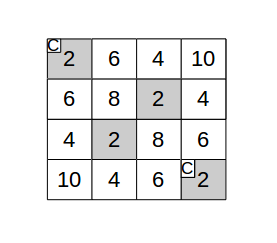
\includegraphics[scale=0.5]{show_solution.png}
		\label{fig:p2_complejidad_varia_k}
	\end{minipage}
\end{figure}

\subsection{Resolución}
Nosotros modelamos el problema con grafos con lo cual resultó equivalente al de camino mínimo 
con un origen y múltiples destinos en un grafo no dirigido sin peso en las aristas. 
En este caso en particular las aristas no tienen peso porque el salto de un caballo siempre 
tiene el mismo costo. En un grafo con las características mencionadas el algoritmo de 
Breadth First Search (TODO agregar cita) obtiene el camino mínimo entre el origen tomado y el resto de los nodos,
éste es el camino entre el origen y el nodo en árbol generado.
El modelo consiste en tomar a las casillas del tablero como nodos del grafo, las casillas en las que 
hay caballos como nodos origen y existe una arista entre dos nodos, casillas, si de una a la otra se
puede ir con un salto de caballo. Cabe destacar que el salto de caballo es simétrico: si con un salto
de caballo se puede ir de la casilla $a$ a la $b$ entonces necesariamente también se puede con un 
salto de caballo ir de la casilla $b$ a la $a$:\\
\begin{figure}[H]
	\begin{minipage}[t]{0.5\linewidth}
		\centering
		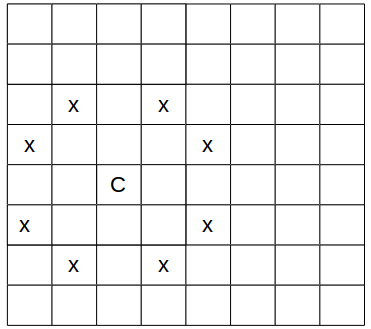
\includegraphics[scale=0.5]{show_jumps.png}
		\label{fig:p2_complejidad_varia_k}
	\end{minipage}
	\begin{minipage}[t]{0.5\linewidth}
		\centering
		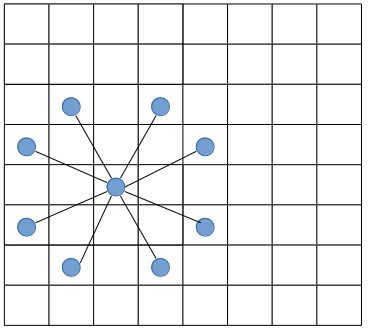
\includegraphics[scale=0.5]{show_graph.png}
		\label{fig:p2_complejidad_varia_k}
	\end{minipage}
\end{figure}
Los pasos para resolver el problema una vez modelado son bastante directos:
\begin{enumerate}
  \item Recorrer el grafo una vez por cada caballo presente tomando como origen el nodo, casilla, en la 
    que se encuentra el caballo.
  \item Guardar, en cada nodo, la cantidad de saltos que le toma a cada caballo llegar a él.
  \item Recorrer todos los nodos y quedarse con alguno de los de suma mínima.
\end{enumerate}
Hay un conjunto pequeño de instancias para los cuales la solución del problema es trivial:
\begin{description}
  \item[$n = 1$] los caballos sólo pueden estar en una casilla por lo cual la solución es la única casilla
    que existe y la cantidad de movimientos totales es 0.
  \item[$n = 2$] los caballos no pueden realizar movimiento permitido alguno. Sólo existe solución en el caso
    en el que los caballos se encuentran todos en la misma casilla.
  \item[$n = 3$] existe solución siempre excepto cuando un caballo comienza en la casilla central del tablero
    en cuyo caso no tiene movimientos permitidos y del resto de las casillas no existe forma de llegar a la
    casilla central mediante movimientos permitidos, lo cual es trivial si vemos que desde la casilla central
    no existen movimientos permitidos porque como ya mencionamos los movimientos del caballo son simétricos.
  \item[$n > 4$] se puede probar fácilmente que de cualquier casilla del tablero se puede acceder a cualquier otra,
    por lo tanto cuando la dimensión del tablero es mayor a 4 siempre existe solución.
\end{description}
En el pseudocódigo no mostramos el manejo de instancias que poseen un tablero de dimensión menor a 4 porque
al ser muy particulares no aportan mayor claridad a la presentación de la idea central del algoritmo.

\subsection{Pseudocódigo}
\begin{algorithm}[H]
  \begin{algorithmic}
    %\STATE $\gets$ \WHILE{} \ENDWHILE \IF{} \ELSE \ENDIF
    \STATE $distancias$ $\gets$ Matriz($n$, $n$)
    \STATE $tablero$ $\gets$ Tablero($n$, $n$)
    \STATE $caballos$ $\gets$ Conj($Casilla$)
    \WHILE {$caballos \neq \emptyset$}
      \STATE $origen$ $\gets$ $caballos$.next()
      \STATE BFS($origen$, $tablero$, $distancias$)
    \ENDWHILE
    \STATE ($suma_{min}$, $casilla_{min}$) $\gets$ MIN($distancias$)
    \caption{caballos\_salvajes}
  \end{algorithmic}
\end{algorithm}

\begin{algorithm}[H]
  \begin{algorithmic}
    %\STATE $\gets$ \WHILE{} \ENDWHILE \IF{} \ELSE \ENDIF
    \STATE $nodos_{no visitados}$ $\gets$ Cola
    \STATE push($nodos_{no visitados}$, $origen$)
    \STATE $tablero_{origen}$ $\gets$ 0
    \STATE $vecinos$ $\gets$ Cola
    \WHILE {$nodos_{no visitados} \neq \emptyset$}
      \STATE $nodo_{actual}$ $\gets$ pop($nodos_{no visitados}$)
      \STATE $vecinos$ $\gets$ obtener\_vecinos($nodo_{actual}$)
      \WHILE {$vecinos \neq \emptyset$}
        \STATE $vecino$ $\gets$ pop($vecinos$)
        \IF {$neg$ esta\_marcado($tablero$, $vecino$)}
          \STATE $tablero_{vecino}$ $\gets$ $tablero_{nodo_{actual}}$+1
          \STATE $distancias_{vecino}$ $\gets$ $distancias_{vecino}$ + $tablero_{vecino}$
          \STATE push($nodos_{no visitados}$, $vecino$)
        \ENDIF
      \ENDWHILE
    \ENDWHILE
    \caption{BFS}
  \end{algorithmic}
\end{algorithm}

\subsection{Demostración de correctitud}
Una instancia del problema está dada por la dimensión del tablero $n$ y la posición
de los $k$ caballos. Luego de modelarlo tenemos un grafo $G = (V, E)$ tal que $\left\vert{V}\right\vert = n^2$, uno
por cada nodo, y $\left\vert{E}\right\vert < n^2 * 4$. La cota superior sobre las aristas proviene del hecho de que
un caballo sólo pude saltar a 8 casillas diferentes como máximo, asumiendo que todos los
saltos posibles caen dentro del tablero. Por lo tanto, la cantidad de aristas debe ser menor
a $\frac{n^2 * 8}{2}$ porque en muchas casillas, como las de las esquinas o las de las bandas, la
mayoría de los saltos posibles caen fuera del tablero. Los caballos los representaremos con un multiconjunto
de nodos al que llamaremos $origenes$, $\left\vert{origenes}\right\vert = \left\vert{caballos}\right\vert = k$. Utilizamos un multiconjunto 
para representarlos porque inicialmente puede haber más de un caballo en una casilla determinada.
Sea $PS_{v,u}$ el conjunto de los caminos posibles entre el nodo $u$ y el nodo $v$.
Dado un nodo $v$ el conjunto de soluciones posibles asociado a $v$ es $SP_v$:
\begin{displaymath}
  SP_v = \left\{ { \sum_{u \in origenes} \left\vert{P_{u,v}}\right\vert : P_{u, v} \in PS_{u, v}} \right\}
\end{displaymath}
La solución óptima para un nodo $v$ la denominaremos $SP_v^{opt}$ y está determinada de la siguiente forma:
\begin{displaymath}
  SP_v^{opt} = \min \left\{ {s : s \in SP_v} \right\} 
\end{displaymath}

\begin{lema}
\label{lema_p2}
Una solución óptima para un nodo $v$ está compuesta por caminos mínimos entre los orígenes
y $v$:
\begin{displaymath}
  s = SP_v^{opt} \Leftrightarrow s = \sum_{u \in origenes} \min \left\{ { \left\vert{P}\right\vert : P \in PS_{u, v}} \right\}
\end{displaymath}
\end{lema}
\begin{proof}
  Sea $SP_{opt}$ una solución óptima para el nodo $v$ que contiene un camino $P_{w,v}$ no mínimo. Sea $P_{w,v}^{min}$ 
un camino mínimo entre $w \in origenes$ y $v$. Sea $SP'_{opt}$:
\begin{displaymath}
SP'_{opt} = SP_{opt} \setminus P_{w, v} \cup \left\{{P_{w,v}^{min}}\right\}
\end{displaymath}
veamos el costo de $SP'_{opt}$ expresado en función del de $SP_{opt}$:
\begin{displaymath}
  SP'_{opt} = \sum_{u \in origenes} \left\vert{P_{u,v}}\right\vert - \left\vert{P_{w,v}}\right\vert + \left\vert{P_{w,v}}\right\vert
\end{displaymath}
pero dado que $P_{w,v}$ no es mínimo:
\begin{displaymath}
  P_{w,v} > P_{w,v}^{min} \Rightarrow P_{w,v} - P_{w,v}^{min} > 0
\end{displaymath}
pero entonces volviendo a la ecuación anterior nos queda que:
\begin{displaymath}
  SP'_{opt} < SP_{opt}
\end{displaymath}
Lo cual es absurdo porque partimos suponiendo que $SP_{opt}$ era un solución óptima y por lo tanto mínima.
\end{proof}

Finalmente, caracterizaremos a la solución del problema $S$:
\begin{displaymath}
  S = \min_{v \in V} \left\{ {SP_{v}^{opt}} \right\}
\end{displaymath}
Nuestro algoritmo calcula el peso del camino mínimo entre cada uno de los orígenes y el resto de los nodos (TODO agregar cita
al cormen capítulo 22 página 598). 
Luego suma en cada nodo $v$ el peso de los caminos mínimos desde cada uno de los orígenes hasta él que por \textbf{Lema 1} es
igual a $SP_{v}^{opt}$. Por último, recorre todos los nodos y toma el mínimo entre todos los $SP_{v}^{opt}$ calculados
lo cual es precisamente la solución que acabamos de definir.

\subsection{Análisis de complejidad}
El algoritmo tiene 3 partes importantes a considerar con respecto a su complejidad:
\begin{enumerate}
  \item generar el grafo que modela la instancia del problema
  \item aplicar BFS una vez por cada caballo con el nodo correspondiente al caballo como origen
  \item buscar el nodo que cuente con la suma mínima
\end{enumerate}
Generar el grafo que modela la instancia del problema recibida tiene costo $O(\left\vert{V}\right\vert) = O(n^2)$. 
Sólo precisamos una matriz de tamaño $n \times n$. Cada posición representa a un nodo y en él almacenaremos la suma
de los caminos mínimos desde cada uno de los caballos hasta él. No es necesario guardar información acerca de las
aristas del grafo porque, al ser el salto de del caballo un movimiento conocido, dado un nodo se pueden obtener sus vecinos
en tiempo constante $O(1)$ calculándolos \textit{ad hoc}:
\begin{center}
(TODO insertar imagen de un tablero con una C en el centro, otra en un rincón y otra en una banda, indicando en cada
caso los saltos posibles)
\end{center}
Tampoco es necesario guardar la distancia desde cada origen hasta cada uno de los nodos ya que sólo nos interesará
la suma total sobre cada nodo. Por lo tanto, basta con ir sumando la distancia de cada uno de los orígenes hasta él.\\
El costo de aplicar BFS es $O(\left\vert{E}\right\vert + \left\vert{V}\right\vert) = O(n^2 * 8 + n^2) = O(n^2)$ (TODO agregar cita al cormen) porque, 
como ya vimos, la cantidad de aristas del grafo está acotada por la cantidad de nodos, porque el caballo a lo sumo
puede saltar a 8 casillas diferentes.\\
Por último, buscar el mínimo tiene un costo $O(\left\vert{V}\right\vert) = O(n^2)$ porque simplemente consiste
en iterar por todos los nodos y quedarse con el que tenga la suma mínima.\\
Por lo tanto, la complejidad está dada por:
\begin{displaymath}
  O(construir\_grafo) + \#caballos * O(BFS) + O(obtener\_minimo) = 
\end{displaymath}
\begin{displaymath}
  O(n^2) + k * O(n^2) + O(n^2) = O(k * n^2)
\end{displaymath}
La cota obtenida $O(n^2 * k)$ es además válida para $\Theta (n^2 * k)$ porque lo único que puede variar de una
instancia a otra del mismo tamaño es la posición de los caballos en el tablero. Sin embargo, la cantidad de nodos
y aristas del grafo es independiente de la posición de los caballos en el tablero. Por lo tanto, el costo de
construir el grafo, recorrerlo con BFS y luego recorrer todos los nodos para obtener el de suma mínima
es el mismo para todas las instancias del mismo tamaño.

\subsection{Tests de complejidad}
El objetivo de las experimentaciones que realizaremos es corroborar que las cotas obtenidas por nuestro análisis
de complejidad son reflejadas por los resultados empíricos. Como la cota depende de la cantidad de caballos
utilizados y las dimensiones del tablero realizaremos dos experimentos:
\begin{enumerate}
  \item Mantendremos la cantidad de caballos ($k$) constante e incrementaremos la dimensión del tablero ($n$) para
    ver si realmente la relación con el crecimiento de la dimensión del tablero es efectivamente cuadrática.
  \item Mantendremos el la dimensión del tablero ($n$) constante e incrementaremos la cantidad de caballos para
    constatar si la relación con la cantidad de caballos es lineal como calculamos.
\end{enumerate}

En el primer experimento variamos la dimensión del tablero desde 1 hasta 100 con un salto de 1. La posición de los
caballos fue elegida pseudo-aleatoriamente, sin restringir que dos caballos tengan la misma posición original.
Para cada dimensión $n$ generamos 10 posicionamientos distintos de los caballos, cada posicionamiento lo ejecutamos
10 veces y nos quedamos con la corrida de menor tiempo de cada posicionamiento para finalmente tomar el promedio
sobre los mínimos de los 10 posicionamientos distintos. Ésto lo realizamos para $k = 5, 10, 15$. El gráfico
que muestra los resultados es el siguiente:
\begin{figure}[H]
	\begin{minipage}[t]{\linewidth}
		\centering
		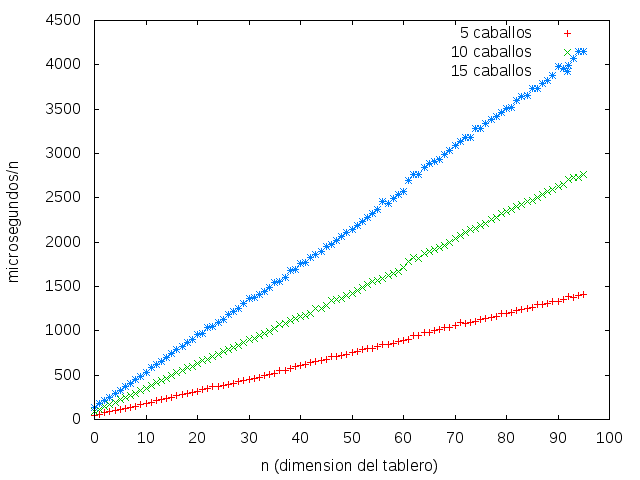
\includegraphics[width=\textwidth]{p2_varia_dimension.png}
		%\caption{}
		\label{fig:p2_complejidad_varia_dimension_tablero}
	\end{minipage}
\end{figure}
Como se ve en el gráfico la cantidad de microsegundos la dividimos por la dimensión del tablero ($n$) y las
curvas resultantes para los 3 casos de caballos se acercan mucho a una recta.

El segundo experimento consistió en tomar un tablero de dimensión fija, en este caso en particular elegimos $n = 40, 70, 100$, y 
variar la cantidad de caballos desde 2 a 50. La posición de los caballos en este caso también fue elegida pseudo-aleatoriamente
y para cada instancia de k caballos la corrimos con 10 posicionamientos distintos de los cuales tomamos el promedio y cada posicionamiento
lo corrimos también 10 veces y nos quedamos con el mínimo. Presentamos los resultados en el siguiente gráfico:
\begin{figure}[H]
	\begin{minipage}[t]{\linewidth}
		\centering
		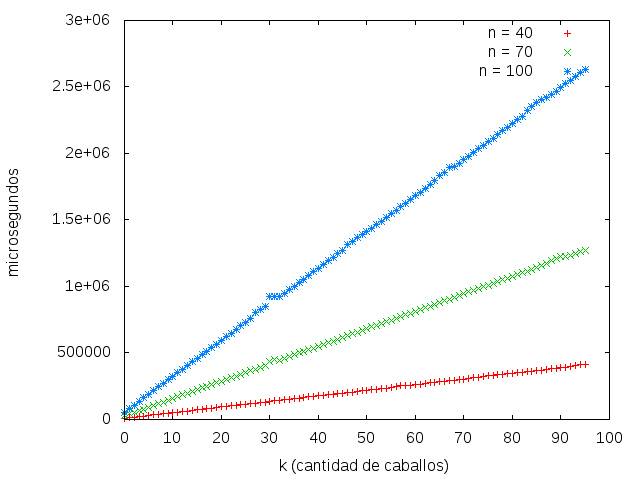
\includegraphics[width=\textwidth]{p2_varia_k.png}
		%\caption{}
		\label{fig:p2_complejidad_varia_k}
	\end{minipage}
\end{figure}

